\documentclass[10pt,mathserif]{beamer}

\usepackage{graphicx,amsmath,amssymb}
\usepackage{listings}
\lstset{language=Python}

%% \input defs.tex

%% formatting
\setbeamertemplate{navigation symbols}{}
\usecolortheme[rgb={0.13,0.28,0.59}]{structure}
\setbeamertemplate{itemize subitem}{--}
\setbeamertemplate{frametitle} {
	\begin{center}
	  {\large\bf \insertframetitle}
	\end{center}
}

\newcommand\footlineon{
  \setbeamertemplate{footline} {
    \begin{beamercolorbox}[ht=2.5ex,dp=1.125ex,leftskip=.8cm,rightskip=.6cm]{structure}
      \footnotesize \insertsection
      \hfill
      {\insertframenumber}
    \end{beamercolorbox}
    \vskip 0.45cm
  }
}
\footlineon

\AtBeginSection[]
{
	\begin{frame}<beamer>
		\frametitle{Outline}
		\tableofcontents[currentsection,currentsubsection]
	\end{frame}
}

%% begin presentation

\title{\large \bfseries Metalearning}

\author{Kris Sankaran\\[3ex]
Mila}

\date{\today}

\begin{document}

\frame{
  \thispagestyle{empty}
  \titlepage
}

\section{Overview}
\begin{frame}
\frametitle{Learning Objectives}
\begin{itemize}\itemsep=12pt
\item Understand basic metalearning setup
\item Recognize metalearning problems ``in the wild''
\item Understand foundational algorithms, on which the rest the
  field stands
\end{itemize}
\end{frame}

\begin{frame}
  \frametitle{Challenge}
  \begin{itemize}\itemsep=12pt
  \item Deep learning methods need lots of data
  \item Humans don't need a million examples of Yaks to be able to recognize
    a new one
  \item How can we have our machines learn from fewer examples?
  \end{itemize}
  \begin{figure}
    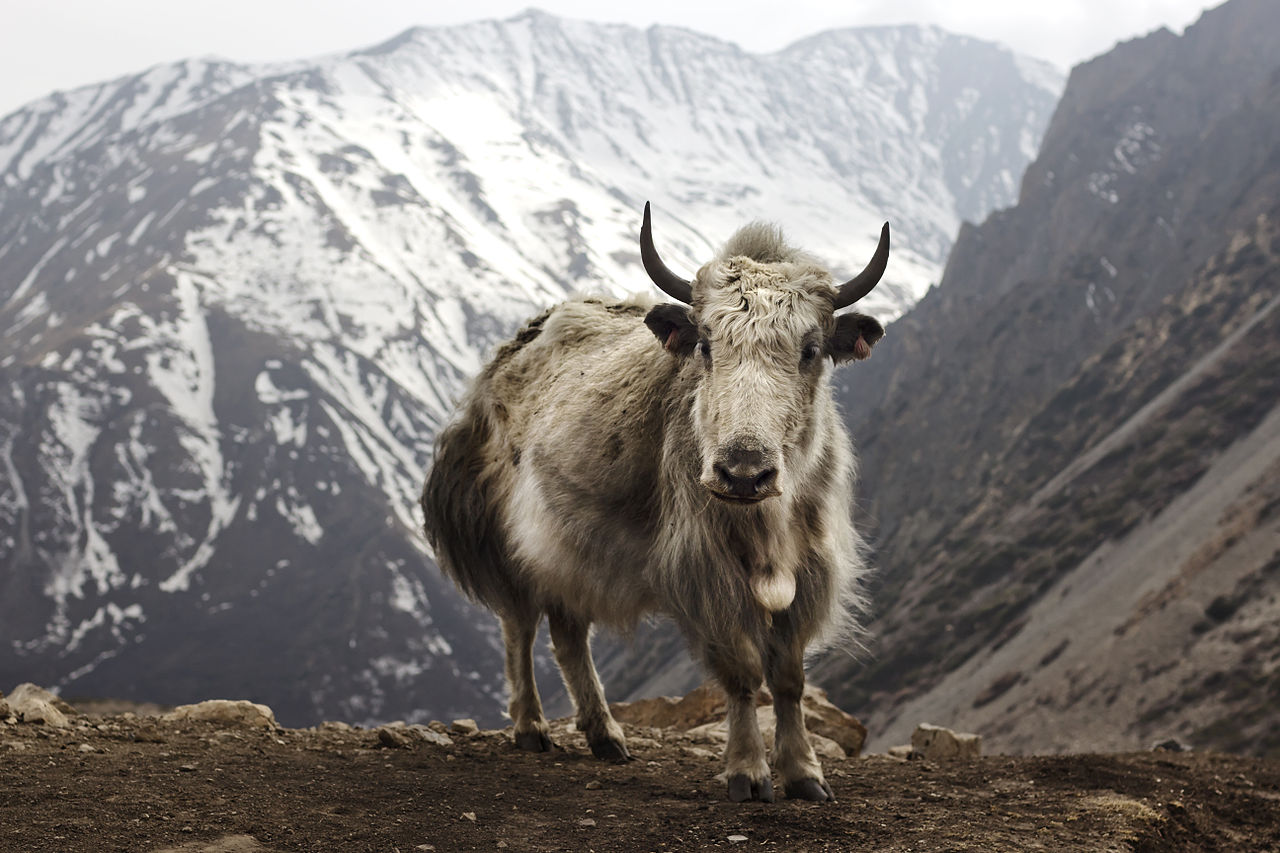
\includegraphics[width=0.4\paperwidth]{figure/yak}
  \end{figure}
\end{frame}

\begin{frame}
  \frametitle{Transfer Learning}
  \begin{itemize}\itemsep=12pt
  \item People figured out a while ago that you can \textit{transfer} to small
    data settings
  \item Train deep model one big dataset, then fine tune the top layers
  \item Bottom layers learn generic visual features
  \end{itemize}
  \begin{figure}
    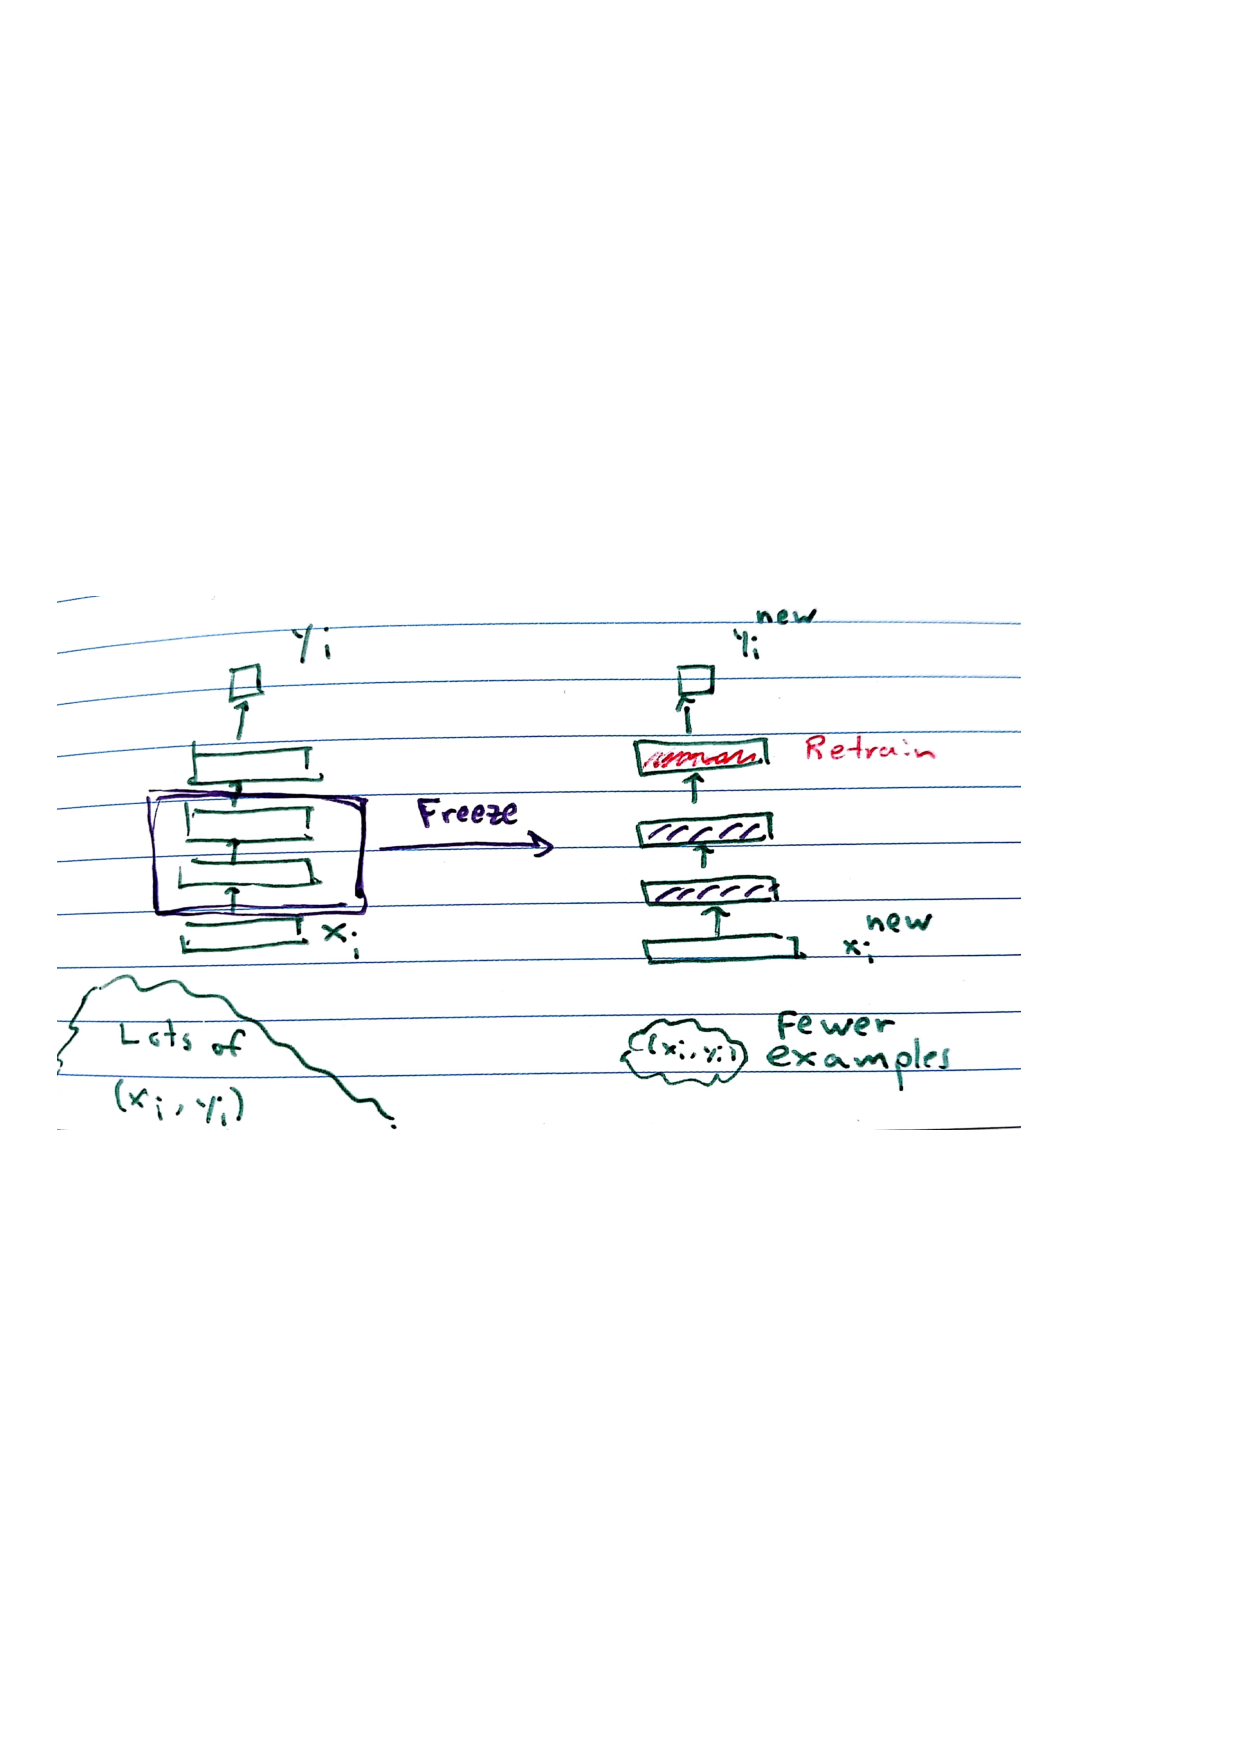
\includegraphics[width=0.6\paperwidth]{figure/transfer_drawing}
  \end{figure}
\end{frame}

\begin{frame}
  \frametitle{Transfer Learning}
  \begin{itemize}\itemsep=12pt
  \item People figured out a while ago that you can \textit{transfer} to small
    data settings
  \item Train deep model one big dataset, then fine tune the top layers
  \item Bottom layers learn generic visual features
  \end{itemize}
  \begin{figure}
    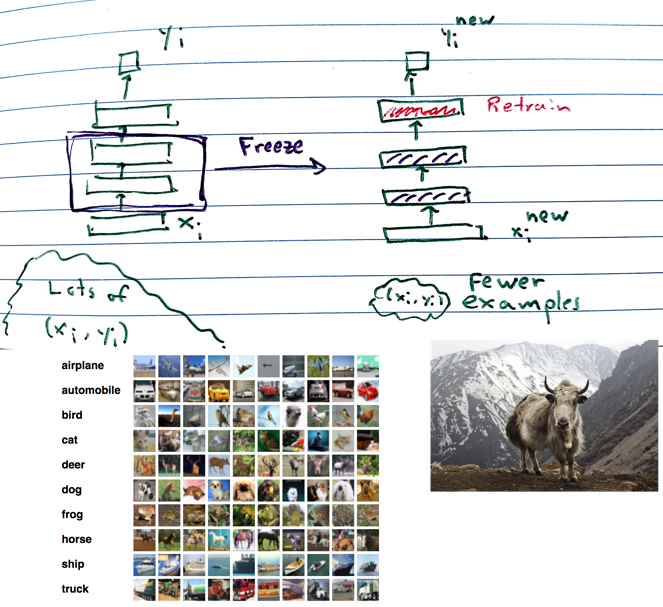
\includegraphics[width=0.6\paperwidth]{figure/transfer_annotated}
  \end{figure}
\end{frame}


\begin{frame}
  \frametitle{Transfer Learning}
  \begin{itemize}\itemsep=12pt
  \item People figured out a while ago that you can \textit{transfer} to small
    data settings
  \item Train deep model one big dataset, then fine tune top layers to scarce
    samples
  \item Bottom layers learn generic visual features
  \end{itemize}
  \begin{figure}
    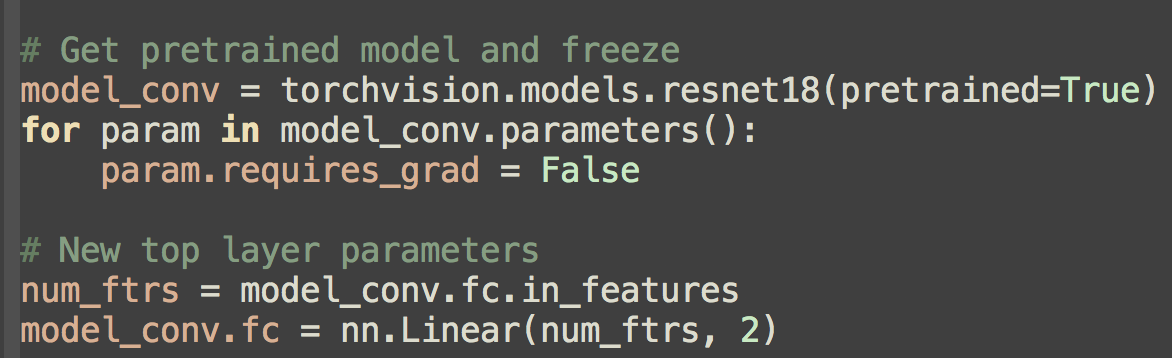
\includegraphics[width=0.8\paperwidth]{figure/transfer.png}
    \caption{From the pytorch transfer learning tutorial}
  \end{figure}
\end{frame}

\begin{frame}
  \begin{itemize}
  \item The same underlying features seem useful across a lot of tasks...
  \item Transfer learning is nice, but lots of hand-tuning
  \item Can we learn models that automatically adapt in scarce data settings?
  \end{itemize}
\end{frame}

\end{document}
